\chapter{Présentation du Projet MoCapIA}

    Maintenant, nous allons présenter le projet MoCapIA en détail, en expliquant les piliers mathématiques sur lesquels il repose, son fonctionnement général. Nous parlerons aussi de l'historique du projet, les travaux accomplis par les précédents stagiaires en détail ainsi que les outils et technologies.

\section{Le processus MoCapIA}
    
    D'après sa définition, la capture de mouvement (motion capture en anglais, parfois abrégé en mocap) est une technique permettant d'enregistrer les positions et rotations d'objets ou de membres d'êtres vivants, pour en contrôler une contrepartie virtuelle sur ordinateur (caméra, modèle 3D ou avatar). Dans notre système, on se focalise sur l'obtention du modèle 3D d'un être humain.
    Il y a 3 étapes principales : la calibration, la détection 2D du corps humain et la reconstruction 3D. Voici un schéma qui résume le projet MoCapIA et son fonctionnement général \textbf{au début du stage} :
    \begin{figure}[H]
        \centering
        
\includegraphics[width=0.8\textwidth]{assets/Capture d'écran process/general/synthèseMOCAPIA.drawio.png}
        \caption{Schéma récapitulatif du fonctionnement général de début de stage}
        \label{fig:fonctionnement_mocapia_debut}
    \end{figure}
    
    \subsection{Partie 1 - Mise en place des caméras et de la calibration}

        Pour capturer le mouvement, nous utilisons 2 à 4 caméras GoPro (précisions dans la partie Outils et Technologies). Ces caméras sont placées autour de la zone de capture de façon à qu'elles aient dans leurs champs de vision une zone commune. Cette zone est l'endroit où l'utilisateur va effectuer son mouvement. Chaque caméra est fixée et ne doit pas bouger durant toute l'expérience (calibration + capture du mouvement). Elles doivent aussi utiliser le même réglage (résolution, fréquence d'images, angle de vue) et doivent être synchronisées entre elles. Pour ça on utilise l'application GoPro qui permet de synchroniser un timecode commun sur les caméras.

        \begin{figure}[H]
            \centering
            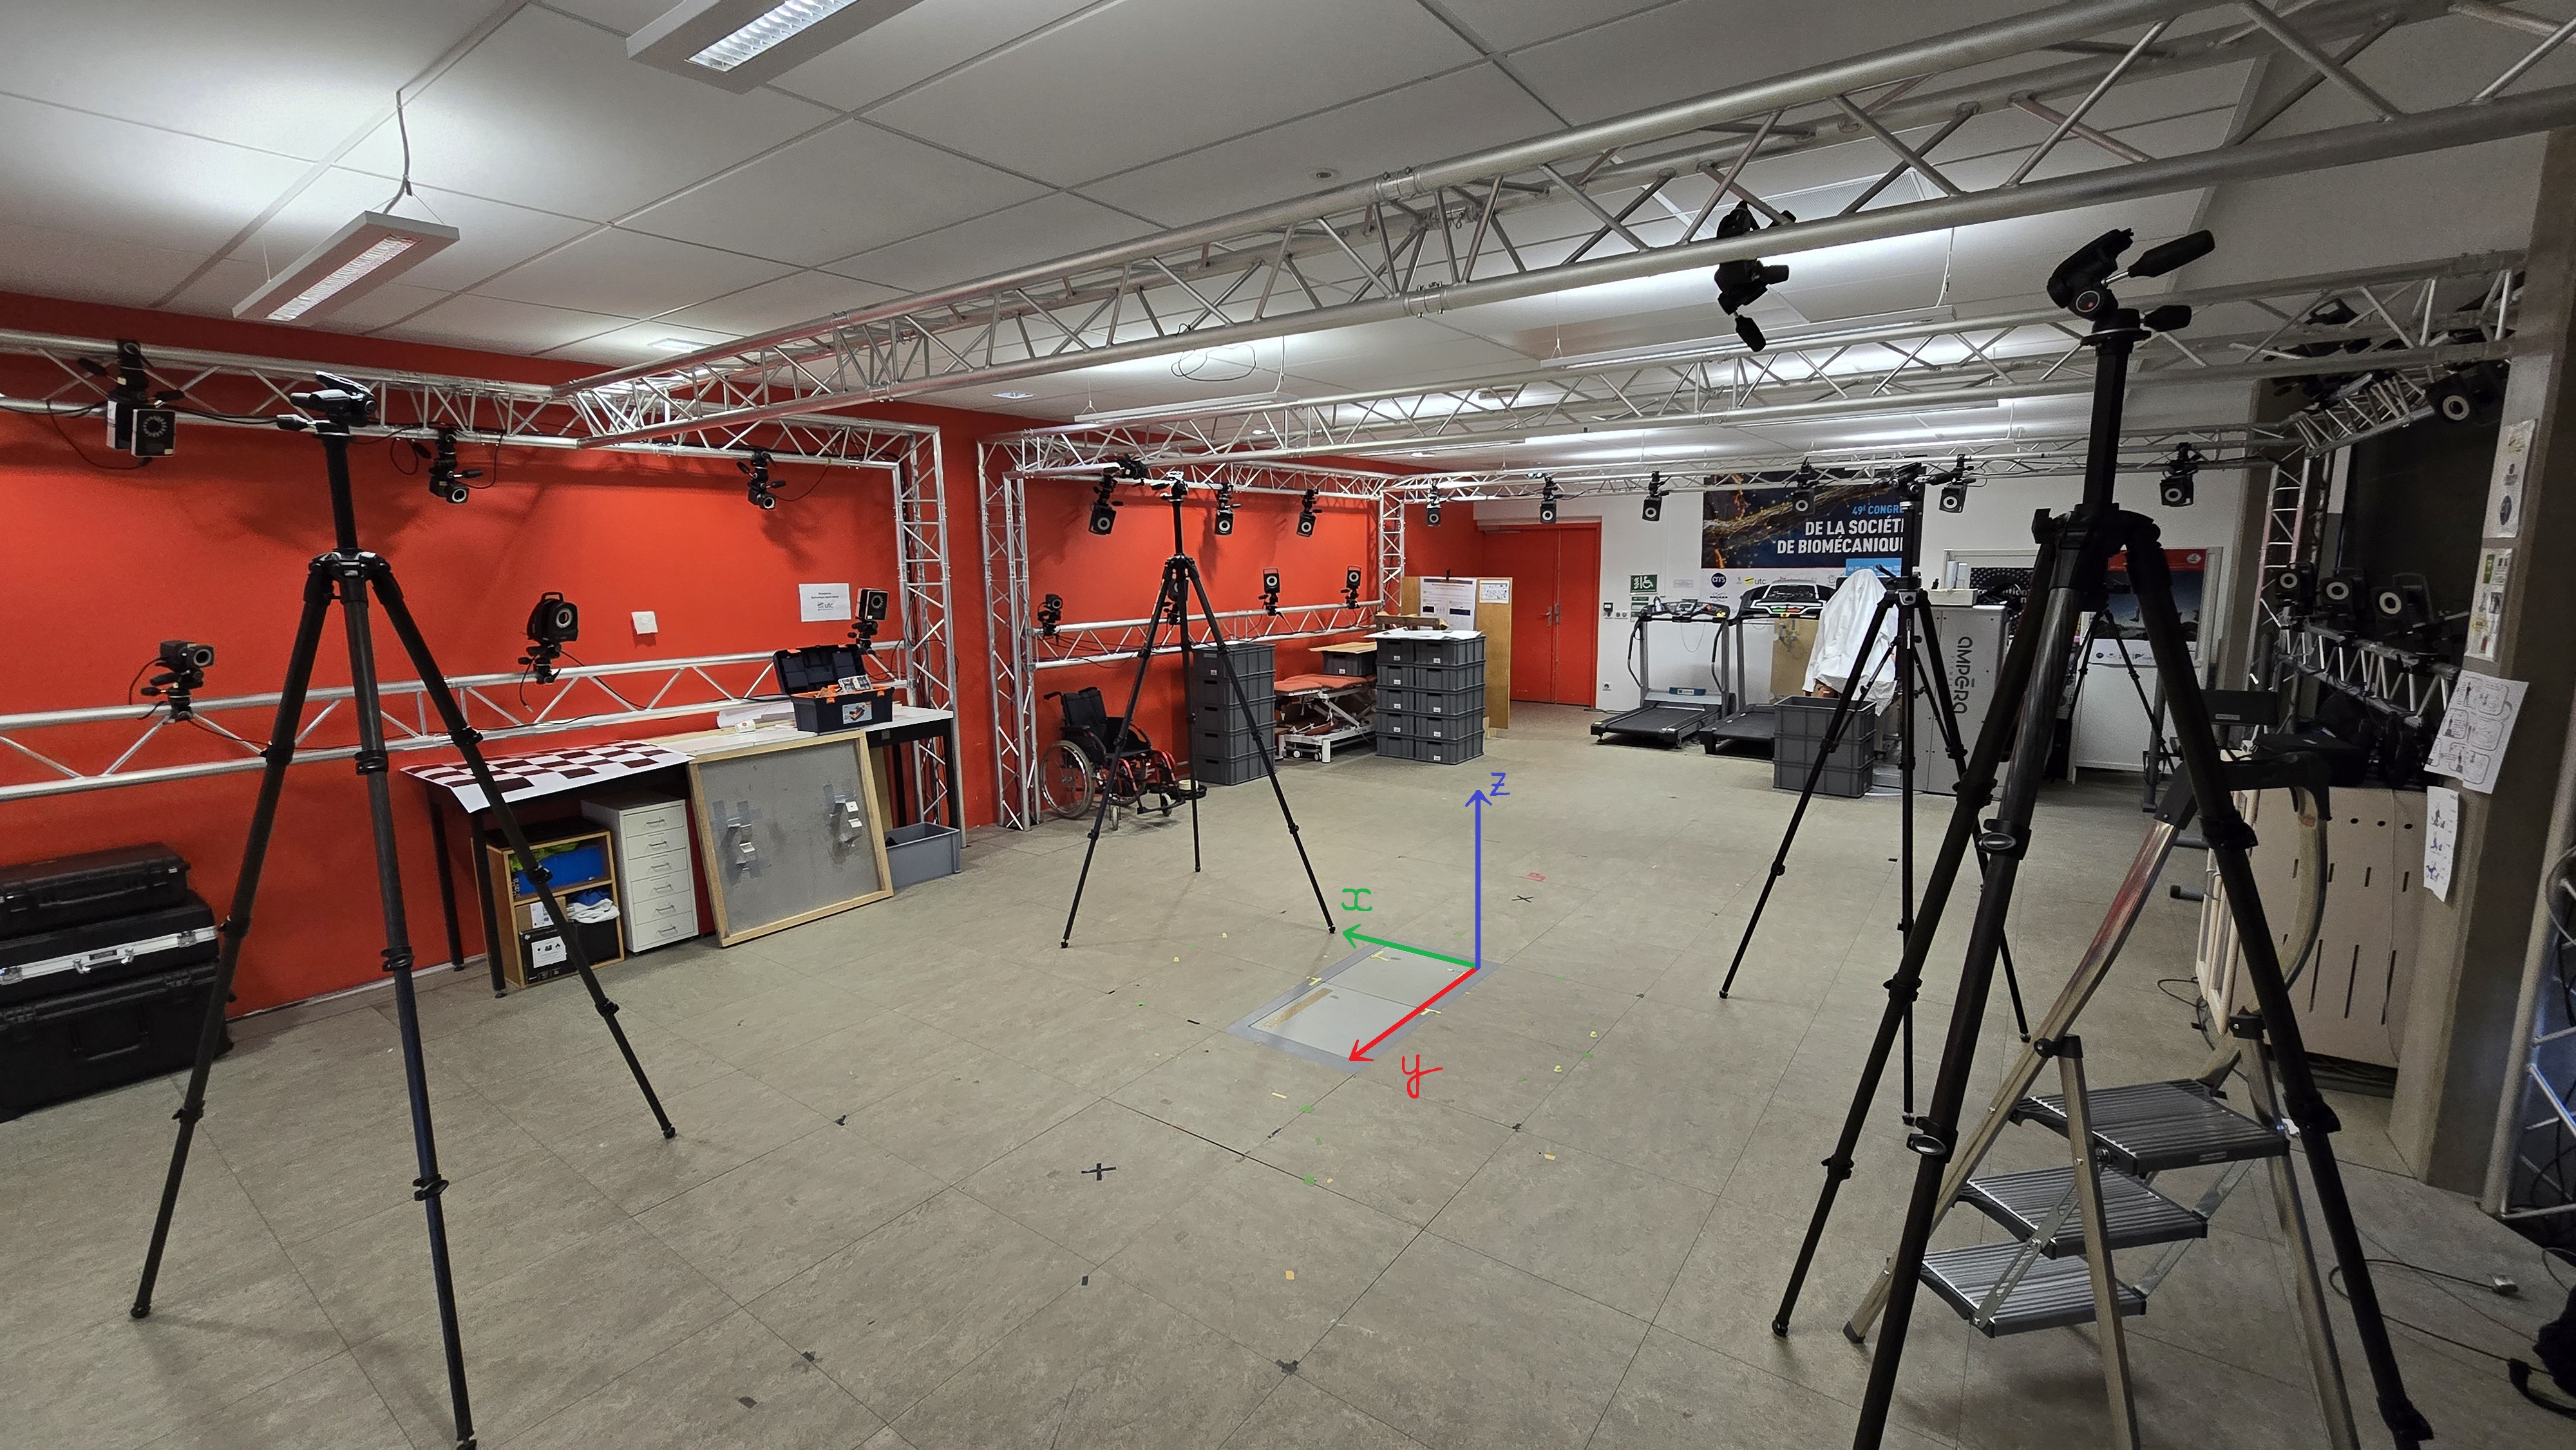
\includegraphics[width=0.8\textwidth]{assets/Capture d'écran process/general/vue trepied.jpg}
            \caption{Mise en place des caméras sur trépied autour de la zone de capture}
            \label{fig:setup_cameras}
        \end{figure}
        Pourtant, avant de capturer le mouvement, on a besoin de calibrer les caméras ce qui est obligatoire avant de vouloir trianguler et obtenir des points 3D. À des fins de compréhension, il est important d'introduire le principe de calibration intrinsèque et extrinsèque \cite{Calibrage}.
        Commençons avec la \textbf{calibration intrinsèque}. Elle consiste à déterminer les paramètres \textbf{internes} à la caméra qui influencent la formation de l'image. Ces paramètres sont fixes donc une fois calculés, ils peuvent être stockés et gardés tant qu'on utilise la même caméra.
        Ces paramètres sont représentés par une matrice $K$ de cette forme :
        $$
        K = \begin{bmatrix}
        f_x & 0 & c_x \\
        0 & f_y & c_y \\
        0 & 0 & 1
        \end{bmatrix}$$
        où :
        \begin{description}
            \item[$f_x$, $f_y$] la focale de la caméra en pixels selon $x$ et $y$
            \item[$c_x$, $c_y$] sont les coordonnées du point d’origine du repère (projection du centre optique sur le plan image)
        \end{description}
        La \textbf{calibration extrinsèque}, quant à elle, définit la position et l'orientation de la caméra dans le repère monde. Les paramètres sont représentés par une matrice de rotation $R \in \mathcal{M}_{3,3}(\mathbb{R})$ et un vecteur de translation $t$. Ces paramètres doivent être recalculés à chaque fois que la caméra est déplacée :
        $$
        [R|t]= \begin{bmatrix}
        r_{11} & r_{12} & r_{13} & t_x \\
        r_{21} & r_{22} & r_{23} & t_y \\
        r_{31} & r_{32} & r_{33} & t_z
        \end{bmatrix} 
        $$ \ref{fig:calibration_cam}
        En appliquant cette matrice $P$ à un point 3D $(X,Y,Z)$ dans le repère monde, on obtient les coordonnées 2D $(u,v)$ dans le repère caméra. Au final, la matrice de projection $P$ de chaque caméra s'obtient en combinant les paramètres intrinsèques et extrinsèques :
        $$
        P = K [R|t]
        $$
        Ces matrices seront utilisées plus tard pour la triangulation des points 3D.
        Dans notre projet l'ensemble de ces informations sont stockées dans un fichier $hdf5$, un format de fichier conçu pour stocker et organiser des données.
        \begin{figure}[H]
            \centering
            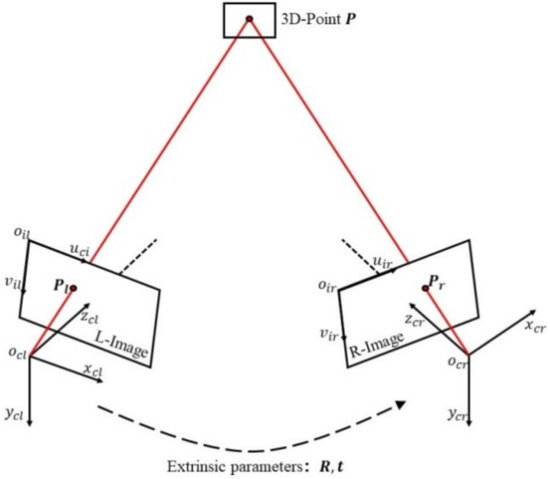
\includegraphics[width=0.7\textwidth]{assets/Capture d'écran process/general/calibration.jpg}
            \caption{Calibration extrinsèque des caméras (cf. \cite{calibraExtrinsic})}
            \label{fig:calibration_cam}
        \end{figure}
        Comme le montre cette figure \ref{fig:calibration_cam}, le repère monde est initialement défini comme le repère 3D de la caméra 1 (ce référentiel sera amené à être changé plus tard).

        \subsection{Estimation de Pose 2D}

        L'estimation 2D du corps humain est l'autre étape importante avant de pouvoir obtenir le modèle 3D final et introduit un aspect essentiel du système : l'Intelligence Artificielle. En effet, comme le projet MoCapIA est un système \textbf{markerless} (sans marqueurs), on identifie les points clés du corps humain grâce à des modèles pré-entraînés. Il en existe plusieurs, chacun ont leurs spécificités, avantages et inconvénients (cette étude a été mené par un ancien stagiaire, voir ...). Nous utilisons une combinaison de deux modèles : YOLO et RTMPose. YOLO (You Only Look Once) est un modèle de détection d'objets en temps réel qui permet de localiser rapidement un objet (ici le corps humain) dans une image. Il assigne à chaque image une carte de classification en fonction des probabilités de présence d'un objet et génère une \textbf{bounding box} (boîte englobante). Il est doté d'un algorithme de tracking qui permet de garder la même bounding box sur le bon sujet durant toute la vidéo.
        \begin{figure}[H]
            \centering
            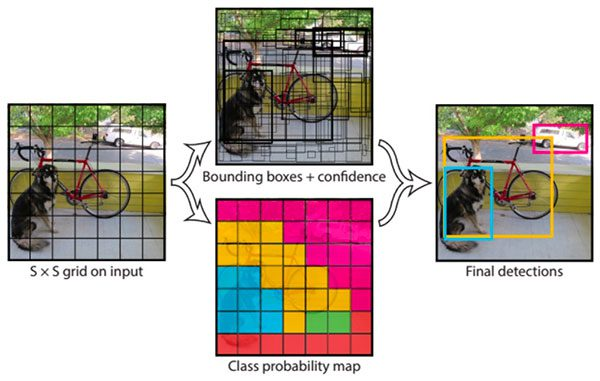
\includegraphics[width=0.7\textwidth]{assets/Capture d'écran process/general/yolo.jpg}
            \caption{Fonctionnement de YOLO (cf. \textit{octo.com})}
            \label{fig:yolo}
        \end{figure}
        Cette étape permet de découper l'image pour ne garder que la partie contenant le corps humain. Ensuite, on utilise le deuxième modèle RTMPose qui est un modèle d'estimation de pose basé sur des (CNN). Il permet de détecter les points clés du corps humain en 2D dans l'image en générant une carte de chaleur, représentant  leur probabilité de présence. Entrainé sur différents squelettes, nous utilisons le modèle Halpe26 qui détecte 26 points clés du corps humain. Les points clés sont stockés dans un fichier .JSON.
        \begin{figure}[H]
            \RawFloats
            \centering
            % --- Figure de Gauche ---
            \begin{minipage}[t]{0.3\textwidth}
                \centering
                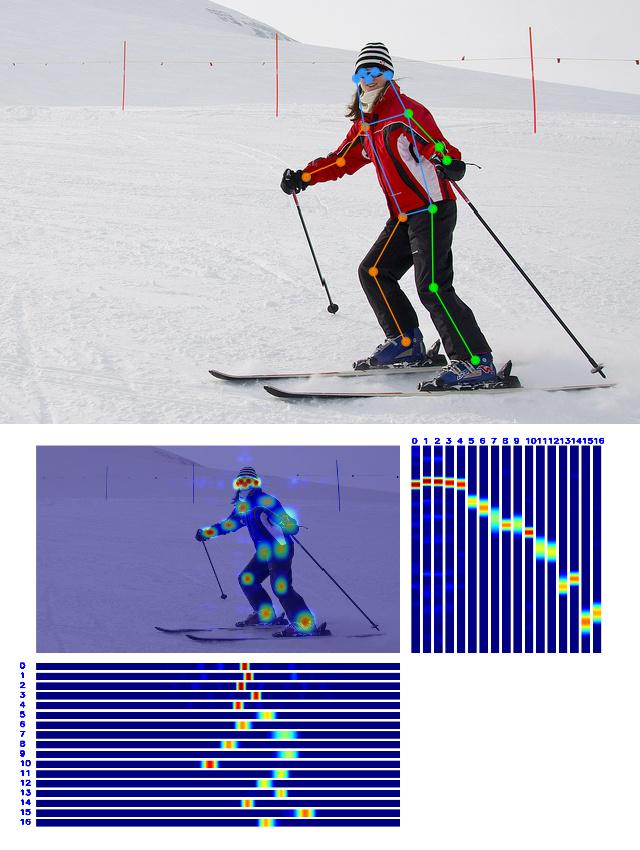
\includegraphics[width=\linewidth]{assets/Capture d'écran process/general/rtmpose.png}
                \caption{Fonctionnement de RTMPose (cf. \href{https://github.com/open-mmlab/mmpose/releases/tag/v1.3.2}{GitHub MMPose})}
                \label{fig:rtmpose}
            \end{minipage}
            \hfill % Espace vital entre les deux
            % --- Figure de Droite ---
            \begin{minipage}[t]{0.5\textwidth}
                \centering
                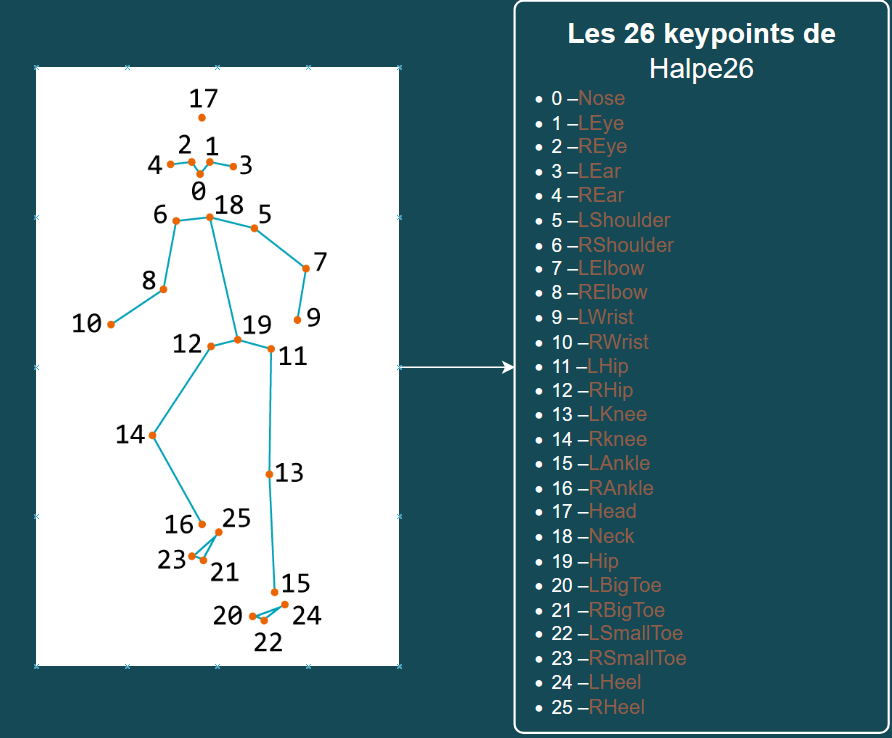
\includegraphics[width=\linewidth]{assets/Capture d'écran process/general/halpe26.png}
                \caption{Modèle Halpe26}
                \label{fig:halpe26}
            \end{minipage}
        \end{figure}
        
    \subsection{Reconstruction 3D}

        Nous disposons maintenant les informations nécessaires pour reconstruire le modèle 3D du corps humain. La première partie de cette reconstruction 3D utilise OpenCV pour trianguler les points 3D à partir de deux premières caméras. Avec un point 2D et les résultats de la calibration de la caméra concernée, on peut tracer une droite dans l'espace 3D partant du centre optique $C$ et passant par le pixel $(u,v)$ projeté en 3D grâce à la matrice intrinsèque $K$ et extrinsèque $R$,$t$ de la caméra :
        $$
        C = -R^{T}t \qquad \text{et} \qquad d = R^{T} \left( K^{-1} \begin{bmatrix} u \\ v \\ 1 \end{bmatrix} \right)
        $$      
        En théorie, pour obtenir la position 3D exacte du point, il suffit d'utiliser une deuxième caméra pour tracer une seconde droite et retrouver l'intersection entre elles. Évidemment dans la réalité les droites ne se coupent pas exactement à cause des erreurs de détection 2D et de calibration. On utilise donc la méthode DLT (Direct Linear Transform) pour minimiser la distance entre les deux droites et obtenir une estimation du point 3D. Disposant de $N$ caméras, on peut générer des candidats pour chaque paire de caméra (figure \ref{fig:triangulation_dlt}). On utilise donc une méthode de \textbf{binning} pour regrouper les candidats dans différents intervalles et renvoie la moyenne de l'intervalle ayant le plus de candidats. Cette méthode permet de réduire l'impact des erreurs de détection et assure une trajectoire 3D plus stable.
        \begin{figure}[H]
            \centering
            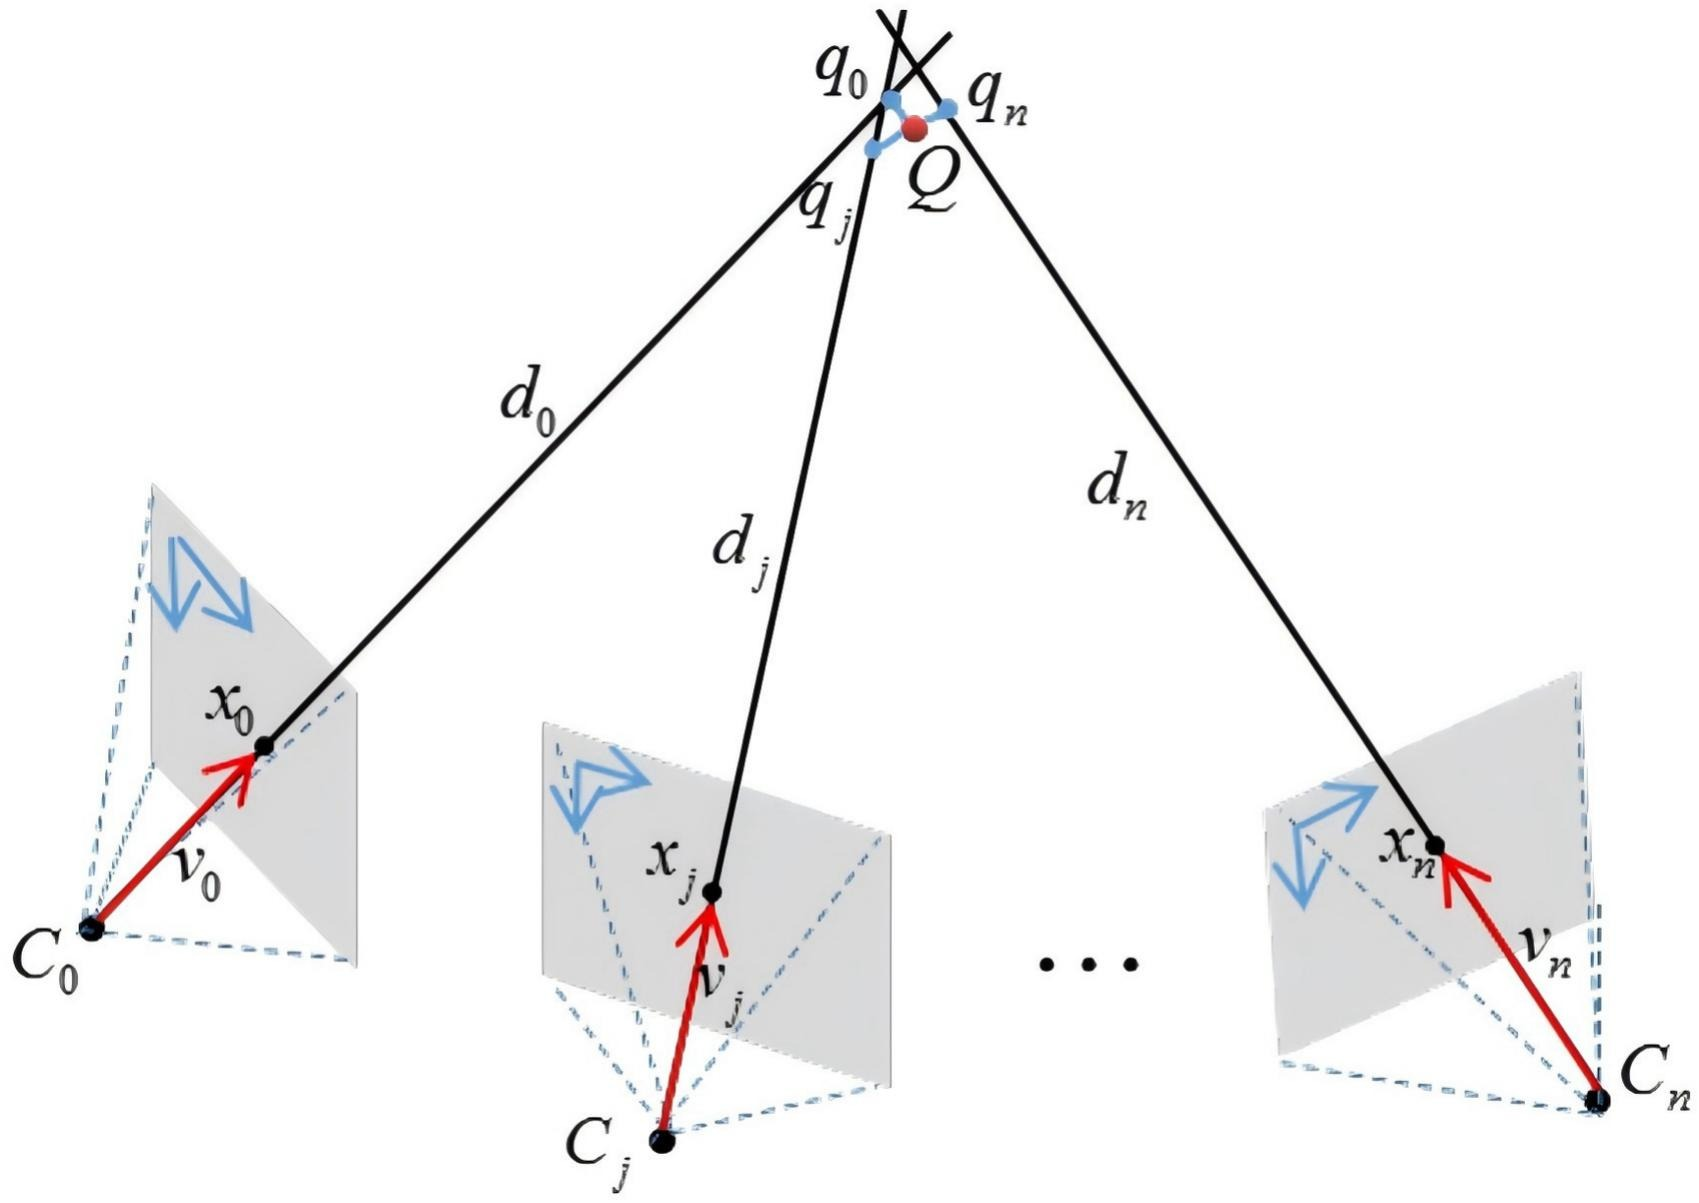
\includegraphics[width=0.8\textwidth]{assets/Capture d'écran process/general/DLT.jpg}
            \caption{Principe de triangulation par DLT (cf. \cite{OrthogonalProjections})}
            \label{fig:triangulation_dlt}
        \end{figure}

        Enfin les coordonnées 3D sauvegardées dans un fichier .CSV sont placés dans le repère monde initial (celui de la caméra 1). Pour mieux pouvoir visualiser et analyser les données, nous devons transformer ce repère dans celui du laboratoire. Pour ça on utilise une transformation rigide (rotation + translation) calculée à partir de points de références 0, X et Y cliqués sur chaque vue des caméras.
        \begin{figure}[H]
            \centering
            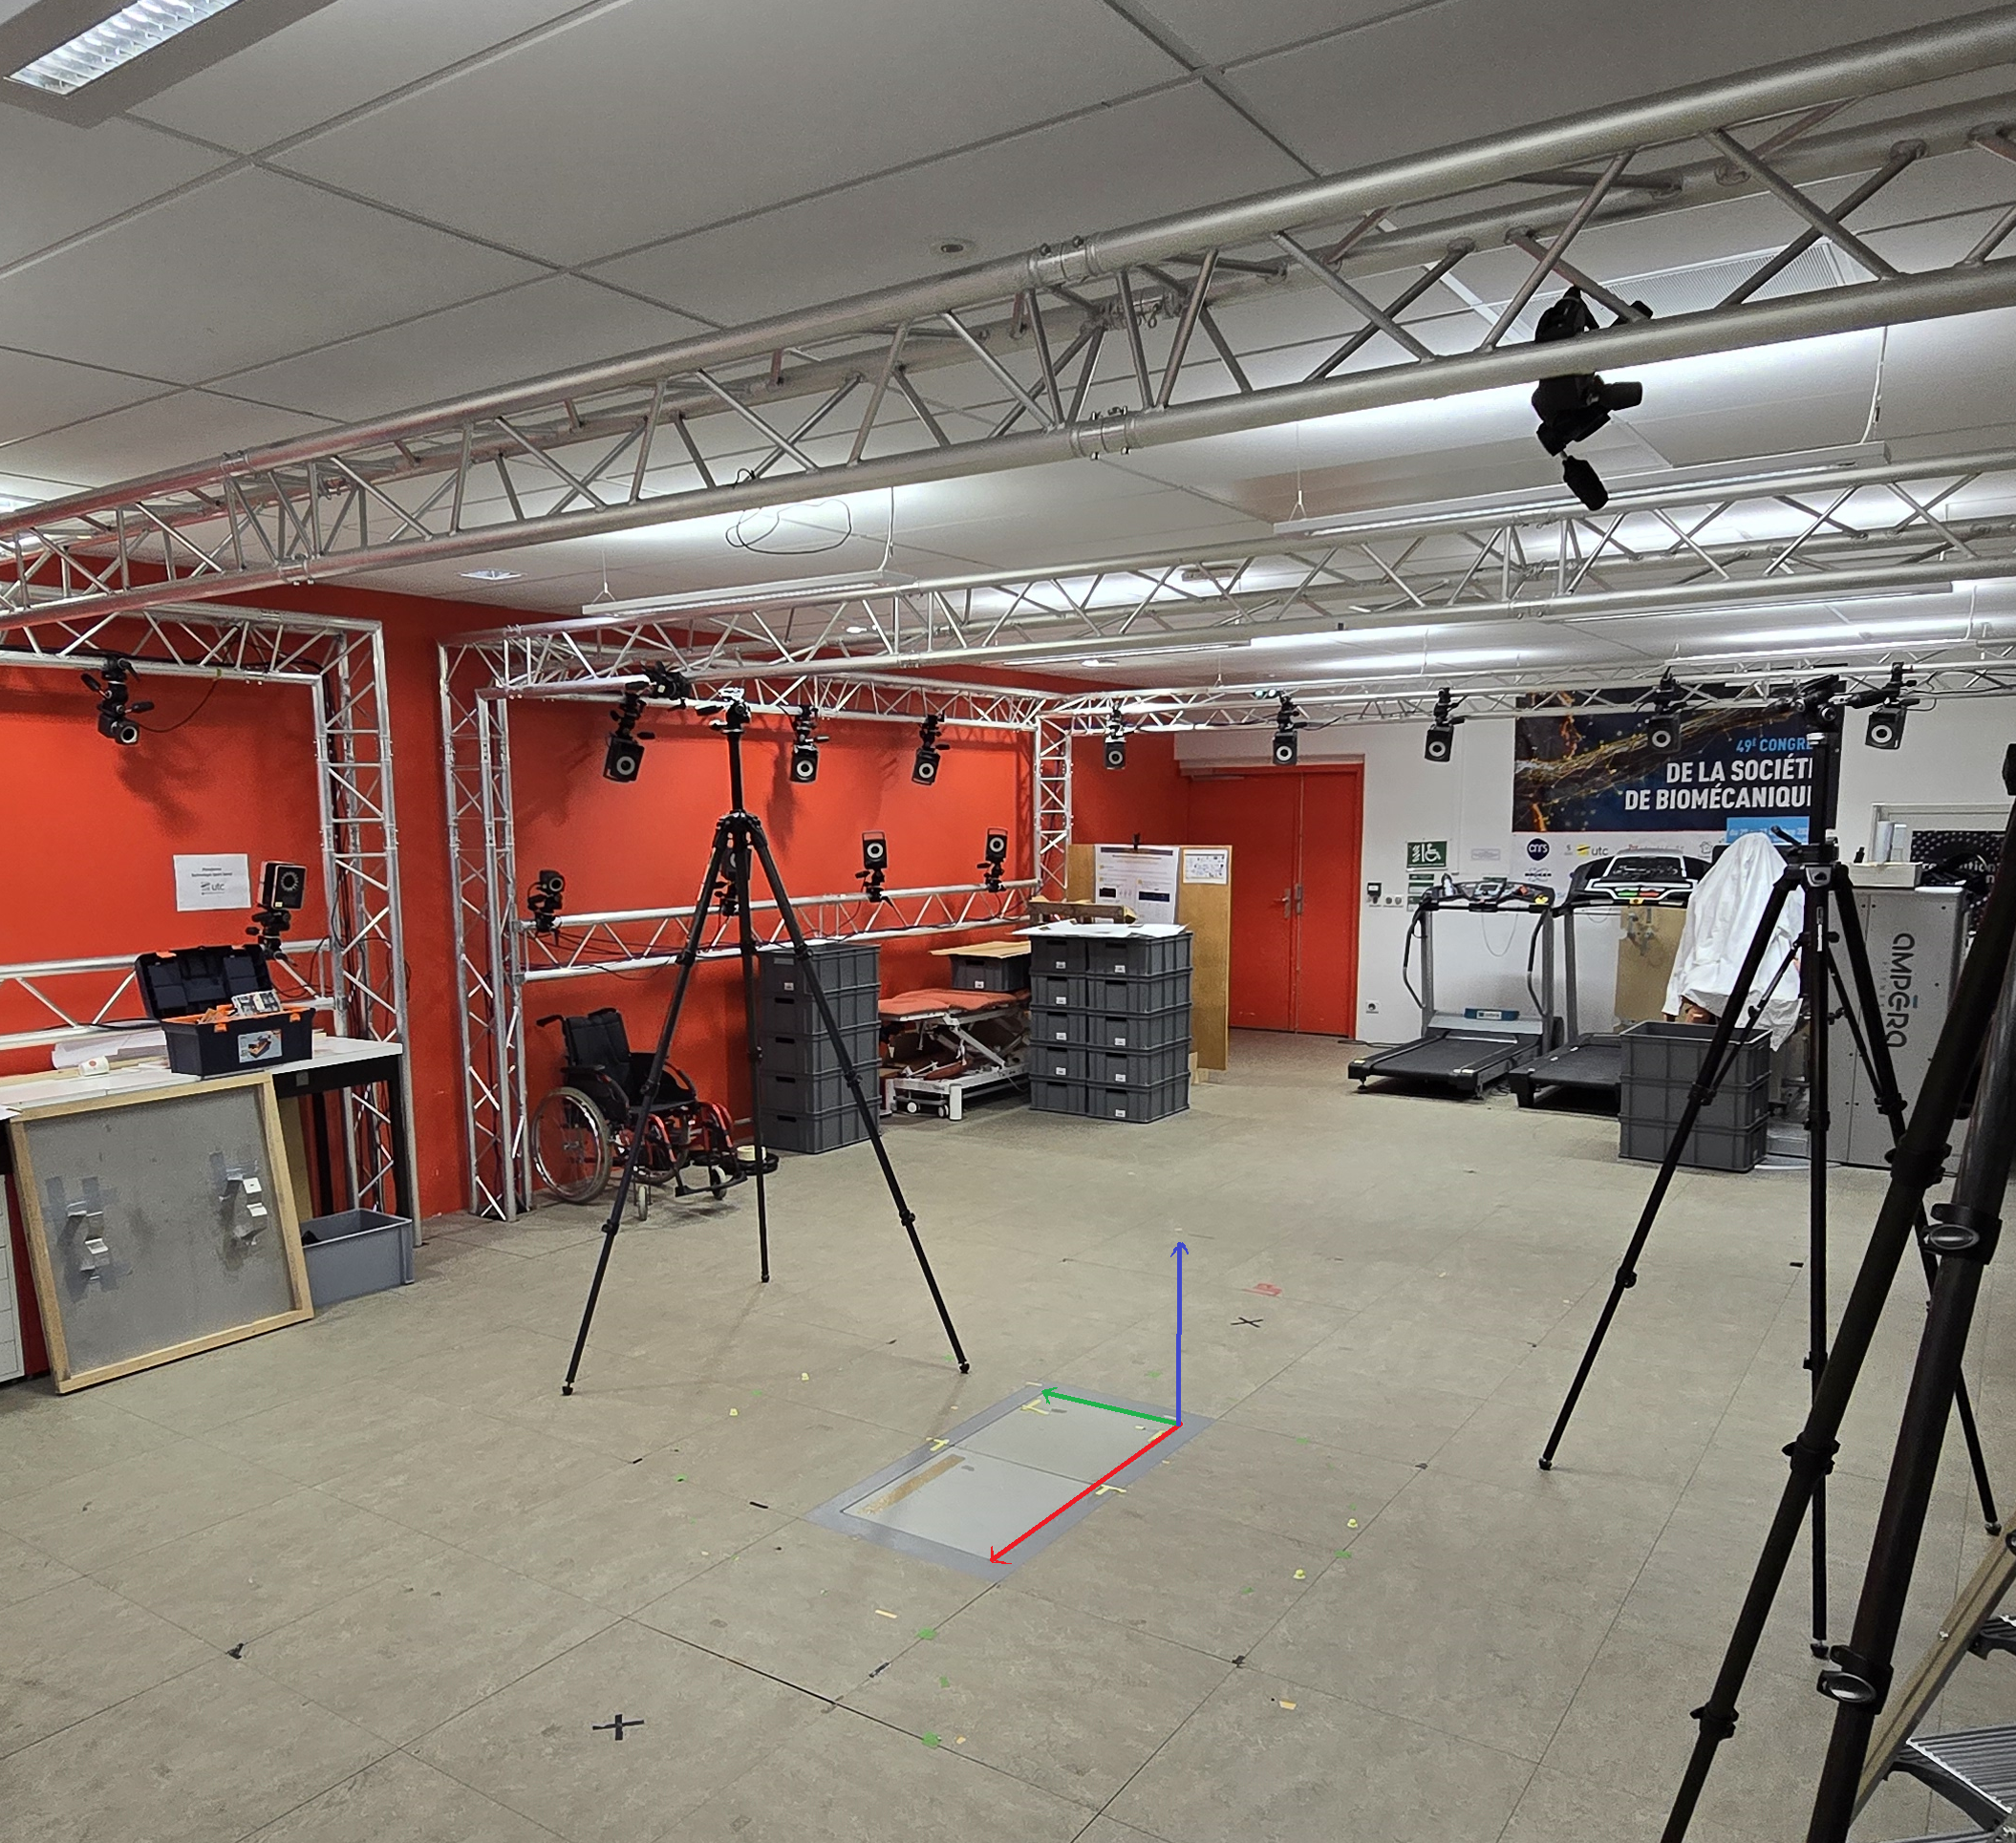
\includegraphics[width=0.8\textwidth]{assets/Capture d'écran process/general/change_ref.png}
            \caption{Changement de repère}
            \label{fig:change_ref}
        \end{figure}

    \subsection{Interface graphique}
        
        Pour l'ensemble de ces étapes, on utilise une interface graphique développée en Python à l'aide la bibliothèque PyQt5. Il permet une utilisation \textbf{user-friendly} ce qui est essentielle pour une future utilisation en milieu clinique ou sportif. En plus de rendre facile la mise en place de la calibration, l'estimation 2D et la triangulation, l'interface permet d'ajouter d'autres fonctionnalités intéressantes :
        \begin{itemize}
            \item \textbf{Structuration des expériences :} Lors de chaque nouvelle expérience, il est possible de créer un nouveau projet, et d'y ajouter un ou plusieurs sujets. Enfin, on peut attribuer à chaque sujet plusieurs sessions de capture.
            \item \textbf{Visualisation du modèle 3D :} Une fois la triangulation terminée, on peut visualiser le fichier CSV (de coordonnées 3D) directement dans l'interface graphique. On a la possibilité d'afficher la distance entre deux points du modèle ou l'angle entre 3 points pour valider ou non la qualité du modèle et permettre l'analyse biomécanique.
            \item \textbf{Lecture des logs :} Durant chaque étape du processus MoCapIA, des logs sont générés pour informer l'utilisateur de l'état d'avancement et d'éventuelles erreurs. L'interface permet de consulter ces logs facilement.
            \item \textbf{Gestion des caméras :} L'interface permet de gérer les caméras GoPro, notamment en choisissant les caméras connectées et leurs réglages (résolution, fréquence d'images, angle de vue).
        \end{itemize}

\section{Historique}

        Comme mentionné précédemment, le projet MoCapIA a été initié en 2023 au semestre d'automne. Jusqu'à maintenant, quatre stagiaires ont travaillé sur le projet, chacun apportant des contributions significatives à son développement. Voici un résumé des travaux accomplis par chaque stagiaire :
        \begin{itemize}
            \item \textbf{Stagiaires 1 et 2 :}
            Les deux premiers stagiaires ont principalement travaillé sur la recherche et l'évaluation des algorithmes et modèles d'IA les plus performants pour réaliser l'estimation de pose 2D en offrant une précision satisfaisante. Même si aucune valeur chiffrée n'a été précisé, le modèle d'IA choisit est considéré comme le plus adapté parmi ceux testés. Les deux critères utilisés pour évaluer les modèles étaient : l'erreur sur les distances et les angles articulaires en comparaison avec le système de référence Vicon, ainsi que la stabilité des points estimés.
            Il existe deux types d'approches dans les algorithmes d'estimation de pose 2D. La première est l'approche \textbf{top-down} qui consiste à d'abord détecter le corps humain dans l'image (généralement avec une bounding box) puis à estimer les points clés à l'intérieur de cette boîte. La seconde approche est \textbf{bottom-up} qui consiste à détecter tous les points clés dans l'image, puis à les regrouper pour former des squelettes complets. Les stagiaires ont conclu que l'approche top-down était plus adaptée pour notre application, car elle offre une meilleure précision et robustesse lors d'expérience avec un faible nombre d'individus tandis que l'approche bottom-up est plus adaptée pour des scènes avec plusieurs. Dans le contexte de MoCapIA, les stagiaires ont privilégié la précision et la robustesse pour un seul sujet. C'est donc l'approche top-down qui a été choisie par l'équipe.
            Parmi les modèles top-down, \textbf{MMPose} est un ensemble d'algorithmes basés sur \textbf{PyTorch}. Accessible via la bibliothèque YOLO, MMPose rassemble plusieurs modèles d'estimation de pose 2D. Après avoir testé plusieurs modèles et en s'appuyant sur une étude menée en 2023 \cite{RTMPose}, les stagiaires ont choisi \textbf{RTMPose} pour sa rapidité et sa précision (cf. \ref{fig:rtmpose_perf}). 
            \begin{figure}[H]
                \centering
                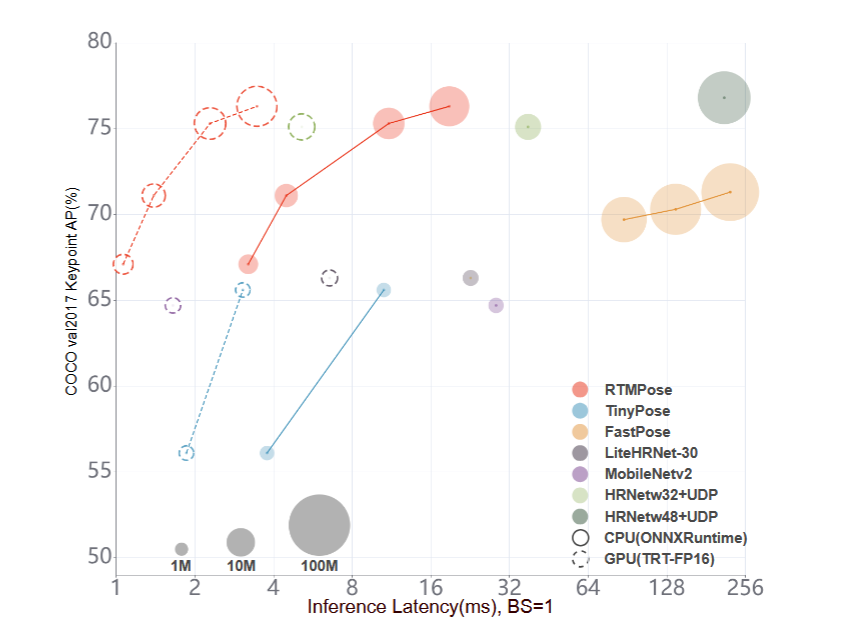
\includegraphics[width=0.8\textwidth]{assets/Capture d'écran process/general/rtmpose_perf.png}
                \caption{Performance de RTMPose comparée à d'autres modèles (cf. \cite{RTMPose})}
                \label{fig:rtmpose_perf}
            \end{figure}
            Il fonctionne en deux étapes : un backbone, suivi d'un détecteur de points clés. Le \textbf{backbone} représente l'architecture principale du modèle (c'est le réseau neuronal convolutif). Il permet l'extraction de caractéristiques sur l'image donc il est en grande partie responsable de la performance du modèle. RTMPose utilise le modèle \textit{ResNet}, qui s'est avéré être  le plus performant. En contrepartie, il est de complexité computationnelle, donc une charge de calcul importante (figure \ref{fig:rtmpose_architecture}). Cette étape est suivie d'un détecteur de points clés qui construit une \textit{heatmap}, représentant les probabilités des positions des points clés. La dernière étape consiste à s'appuyer sur les résultats du backbone et du détecteur pour prédire les positions 2D des points clés du corps humain sous forme de matrice.
            \begin{figure}[H]
                \centering
                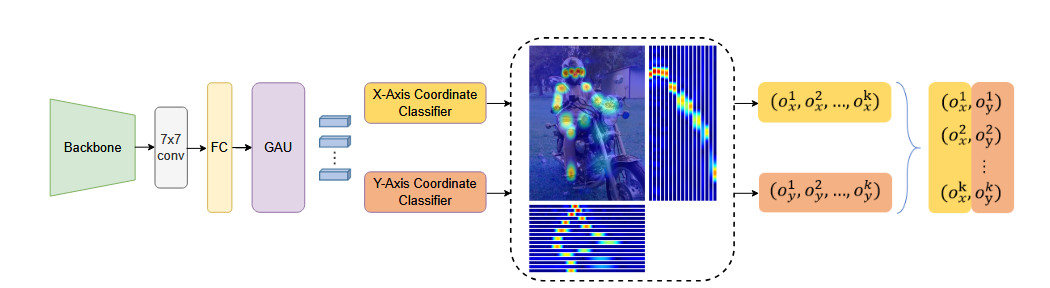
\includegraphics[width=0.8\textwidth]{assets/Capture d'écran process/general/rtmpose_explained.png}
                \caption{Architecture de RTMPose (Han, 2023), un backbone RestNet permet d’extraire les différentes caractéristiques de l’image, puis un détecteur de points clés construit la heatmap des points remarquables du sujet. Ces points sont renvoyés sous la forme d’une matrice (cf. \cite{RTMPose}).}
                \label{fig:rtmpose_architecture}
            \end{figure}
            \item \textbf{Stagiaire 3 :} Durant le semestre A24, le troisième stagiaire a intégré le principe de calibration/triangulation ainsi que l'interface graphique au projet.
            Pour la calibration, la méthode de Zhang (\cite{Zhang}) a été utilisé pour déterminer les paramètres intrinsèques et extrinsèques de chaque caméra. Cette méthode est très flexible et nécessite peu d'image de l'objet de calibration. Ici le choix de l'objet de calibration s'est porté sur un damier 6 lignes x 5 colonnes de case de 120 mm. D'après l'étude, plus un damier possède de cases, plus le nombre d'images nécessaires est faible. étant donné que le nombre de points est plus important. Nous vérifierons cette affirmation plus tard dans le chapitre \ref{Réalisations}. Cette calibration fonctionne pour deux caméras, mais elle a besoin d'être adaptée pour fonctionner avec plus de deux caméras. Pour ça, l'équipe avait mis en place une calibration avec une baguette de calibration 3D, mais les résultats n'étaient pas satisfaisants. Il a donc été décidé de garder la calibration avec damier en le faisant circuler de manière à toujours être visible par au moins deux caméras.

            C'est aussi durant ce stage qu'ont été intégrés l'étape de triangulation et de changement de repère. La méthode retenue est la méthode DLT (Direct Linear Transform) qui permet de minimiser la distance entre les droites issues de chaque caméra, puis une moyenne du résultat de chaque paire afin d'obtenir un résultat plus stable. 

            De plus le principe de \textbf{Multi-Threading} a été implémenté pour accélérer l'ensemble du processus MoCapIA. Son implémentation permet d'effectuer plusieurs tâches en parallèle, optimisant ainsi l'utilisation des ressources du système et réduisant le temps d'attente pour l'utilisateur.
            \begin{figure}[H]
                \centering
                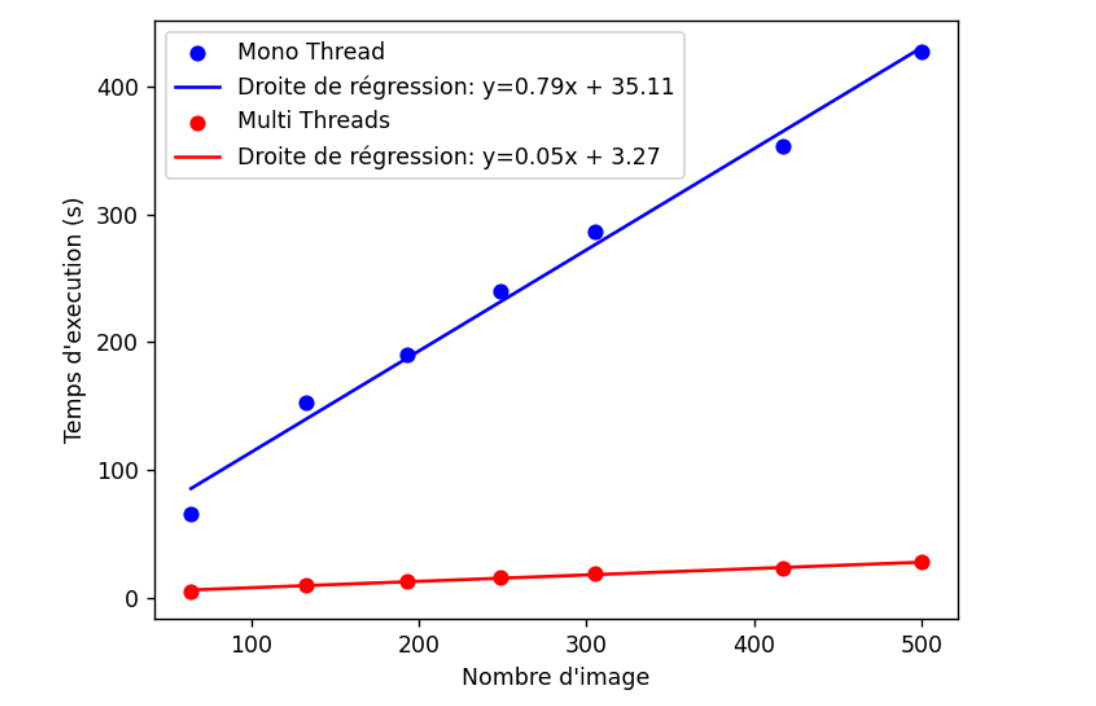
\includegraphics[width=0.8\textwidth]{assets/Capture d'écran process/general/multithread.png}
                \caption{Impact du multi-threading sur le processus MoCapIA}
                \label{fig:multithreading}
            \end{figure}
            Alors que le temps d'exécution en seconde augmente proportionnellement avec le nombre d'images à traiter dans une approche mono-thread, l'approche multithread maintient un temps d'exécution quasi constant. 

            Enfin l'équipe a jugé nécessaire de développer une interface graphique pour rendre le logiciel plus accessible et ergonomique. Pour ça un cahier des charges a été établi pour définir les fonctionnalités et l'apparence de l'interface. Il a donc instauré une structure de fichiers claire et intuitive pour chaque expérience, sujet et session. Les GoPro, utilisables avec différentes résolutions et fréquences d'images, sont maintenant configurables directement depuis l'interface. Le choix s'est porté sur une configuration de projet basé sur trois fichiers .JSON afin de stocker dans un premier les réglages du logiciel (raccourcis, fonctionnalités en option), dans un deuxième les informations relatives au statut du projet et dans un troisième les informations sur les caméras (résolution, fréquence d'images, angle de vue, paramètres intrinsèques, calibration extrinsèque). Graphiquement parlant, le logiciel construit se divisait en deux sections principales. La première section \textit{Acquisition} (figure \ref{fig:interface_colin1}) permet de gérer les expériences, les caméras et surtout de lancer les différentes étapes du processus :
            \begin{figure}[H]
                \centering
                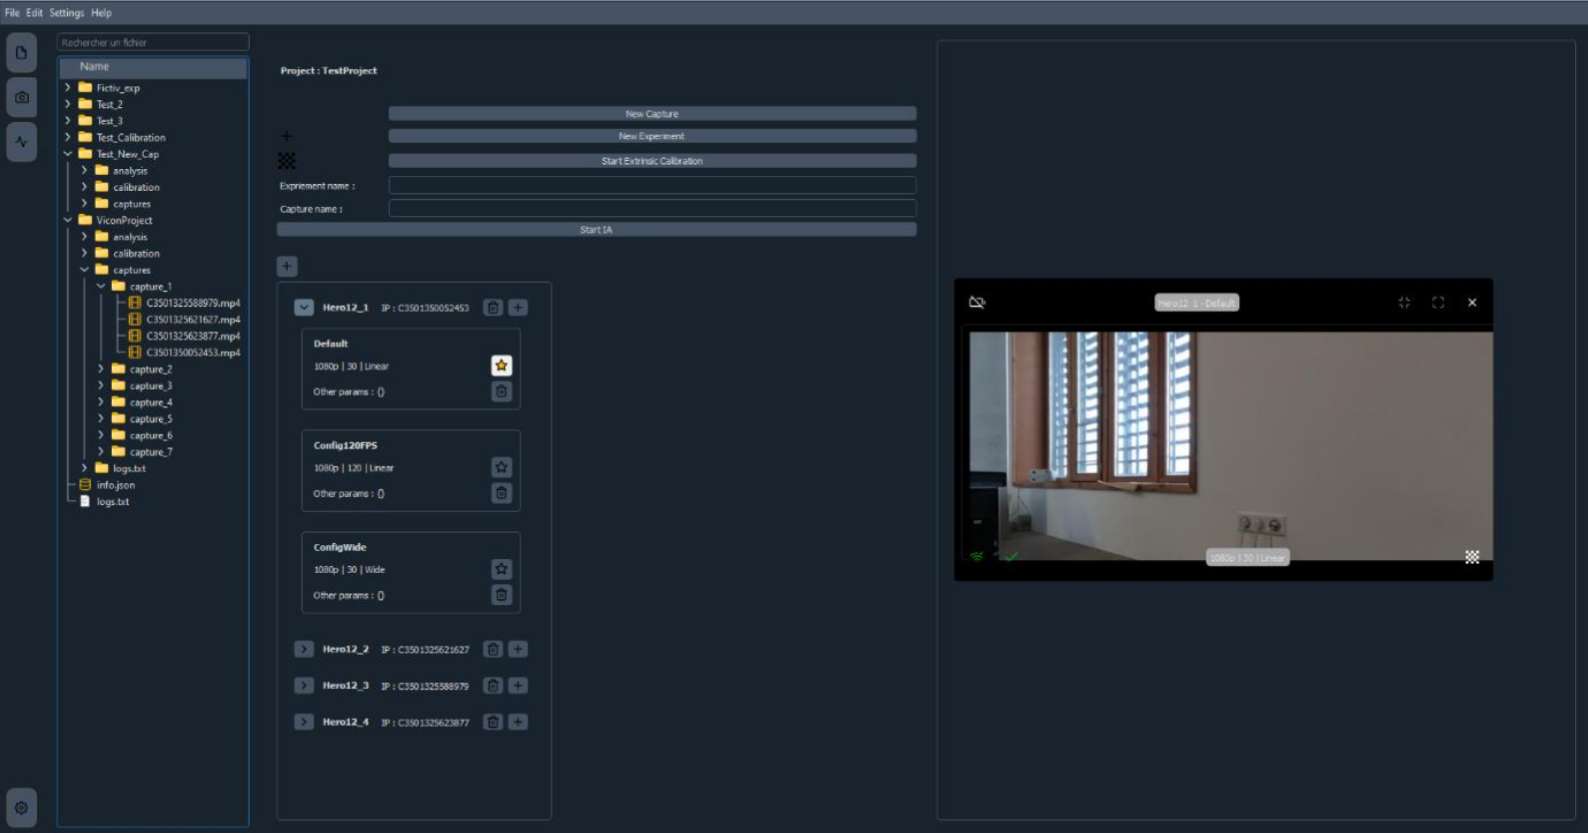
\includegraphics[width=0.8\textwidth]{assets/Capture d'écran process/general/interface_colin1.png}
                \caption{Section 1 de l'Interface graphique développée par le troisième stagiaire}
                \label{fig:interface_colin1}
            \end{figure}
            L'autre aspect important du cahier des charges consistait à permettre la visualisation du modèle 3D directement dans l'interface. C'est pourquoi dans une deuxième section \textit{Visualisation} (figure \ref{fig:interface_colin2}), l'utilisateur peut visualiser le modèle 3D sur le mouvement sélectionné. Il est possible en plus d'afficher les distances entre deux points du modèle ou l'angle entre 3 points pour permettre une analyse biomécanique rapide. C'est le premier grand pas vers une utilisation clinique ou sportive du système MoCapIA. 
            \begin{figure}[H]
                \centering
                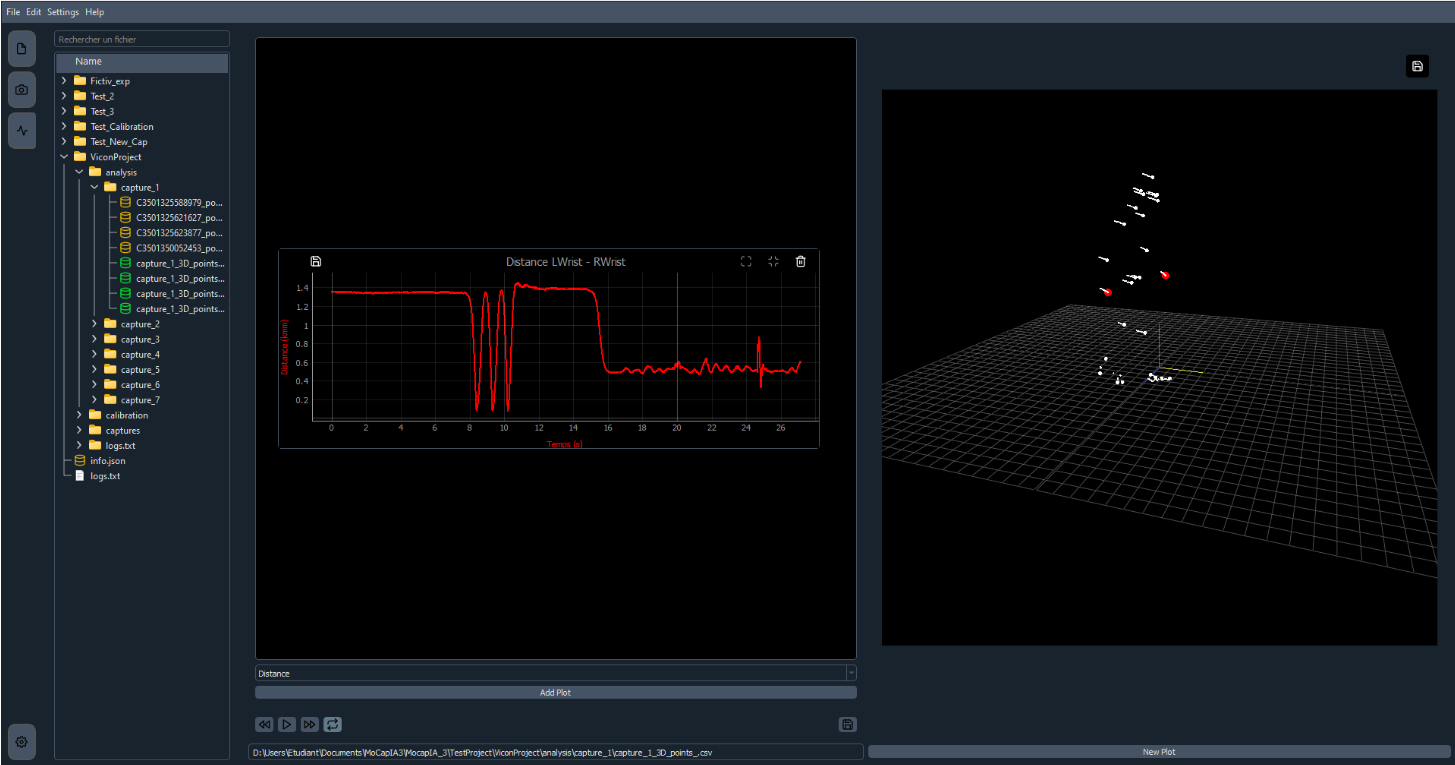
\includegraphics[width=0.8\textwidth]{assets/Capture d'écran process/general/interface_colin2.png}
                \caption{Section 2 de l'Interface graphique}
                \label{fig:interface_colin2}
            \end{figure}
        
            \item \textbf{Stagiaire 4 :} Durant le semestre P25, le quatrième stagiaire a principalement travaillé sur l'optimisation du processus MoCapIA et l'amélioration de l'interface graphique. Un affichage en temps réel de la progression par l'intermédiaire de logs et de barre de progression a été développé ce qui permet de suivre l'avancement de chacune des étapes. 
            Une méthode \textit{binning} a été implémentée dans la triangulation. Cette méthode permet de regrouper les différents points 3D candidats générés par chaque paire de caméras dans des intervalles. Le point final est obtenu en faisant la moyenne des points dans \textbf{l'intervalle ayant le plus de candidats}. Cet ajout rend la triangulation plus robuste face aux erreurs importantes. 
        \end{itemize}

\section{Le planning}

    La mise en place des tâches s'est faite lors de réunion hebdomadaire avec le tuteur de stage et parfois l'ensemble de l'équipe. Pour autant, les échanges étaient beaucoup plus fréquents, donc plusieurs ajustements ont été réalisés en fonction des imprévus et des découvertes faites par le tuteur de stage ou nous les stagiaires. Le planning général est présenté ci-dessous dans le tableau \ref{tab:planning}.

    \begin{table}[h!]
        \centering
        \renewcommand{\arraystretch}{1.5}
        \begin{tabularx}{\textwidth}{|c|c|X|} 
            \hline
            \textbf{Période} & \textbf{Phase} & \textbf{Description} \\
            \hline
            Semaine 1 & Prise en main & Réalisation du processus en entier sur l'ordinateur du précédent stagiaire (Ui, capture du mouvement, calibration, gestion des GoPro) \\
            \hline
            Semaine 2 & Installation & Étant donné que nous sommes deux, il a fallu installer le logiciel sur un nouvel ordinateur pour qu'il puisse lancer le logiciel avec les bonnes versions \\
            \hline
            Semaine 3 & Recherches Bibliographiques & Recherche sur les différentes étapes du processus MoCapIA, compréhension des principes mathématiques et informatiques \\
            \hline
            Semaines 4 à 6 & Tests de calibration & Réalisation de plusieurs tests pour évaluer la qualité de la calibration en fonction de différents paramètres (type de damier, nombre d'images, position des caméras) \\
            \hline
            Semaines 7 à 9 & Recherche sur la triangulation & Étude des différentes méthodes de triangulation et test sur la triangulation globale \\
            \hline
            Semaine 10 & Test de l'estimation 2D & Réalisation de plusieurs tests pour évaluer la qualité de l'estimation 2D en comparaison avec le Vicon \\
            \hline
            Semaines 11 à 14 & Ajout de nouvelles fonctionnalités & Ajout des étapes de filtrage, d'augmentation de marqueur, et de cinématique inversée \\
            \hline
            Semaines 15 à 17 & SAM 3D & Recherche sur le modèle SAM 3D de Meta et réalisation de tests \\
            \hline
            Semaines 18 à 20 & Rapport & Rédaction du rapport de stage \\
            \hline
        \end{tabularx}
        \caption{Répartition des tâches durant le stage}
        \label{tab:planning}
    \end{table}


\section{Outils et Technologies}

    \subsection{Hardware (matériels)}

        \subsubsection{Configuration de l'ordinateur}
        \begin{itemize}
            \item Processeur (CPU) : Intel Core i9-14900K
            \item Mémoire vive (RAM) : 64 Go
            \item Carte graphique (GPU) : NVIDIA GeForce RTX 4090
        \end{itemize}
        Ces composants haut de gammes ont eu un réel impact sur la rapidité d'exécution du processus MoCapIA, notamment grâce à la carte graphique qui permet d'accélérer les calculs liés à l'Intelligence Artificielle.
        
        \subsubsection{Systèmes de caméras}

        \begin{table}[h!]
        \centering
        \renewcommand{\arraystretch}{1.5}
        \begin{tabularx}{\textwidth}{|c|c|X|} 
            \hline
             & \textbf{MoCapIA} & \textbf{Vicon (référence)}\\
            \hline
            Nombre de caméras & 4 caméras GoPro Hero 12 Black \ref{fig:gopro} & 37 caméras infrarouges MXT160, Bonita 3 et Vantage 5 \\
            \hline
            Résolution utilisée & 1080 pixels & 16 mégapixels\\
            \hline
            Images par seconde (ips) & 30 & 120 \\
            \hline
            synchronisation & < 10 microsecondes & < 1 milliseconde (horloge de phase) \\
            \hline
        \end{tabularx}
        \caption{Comparaison des différents systèmes de caméras}
        \label{tab:cameras}
    \end{table}

    \begin{figure}[H]
        \centering
        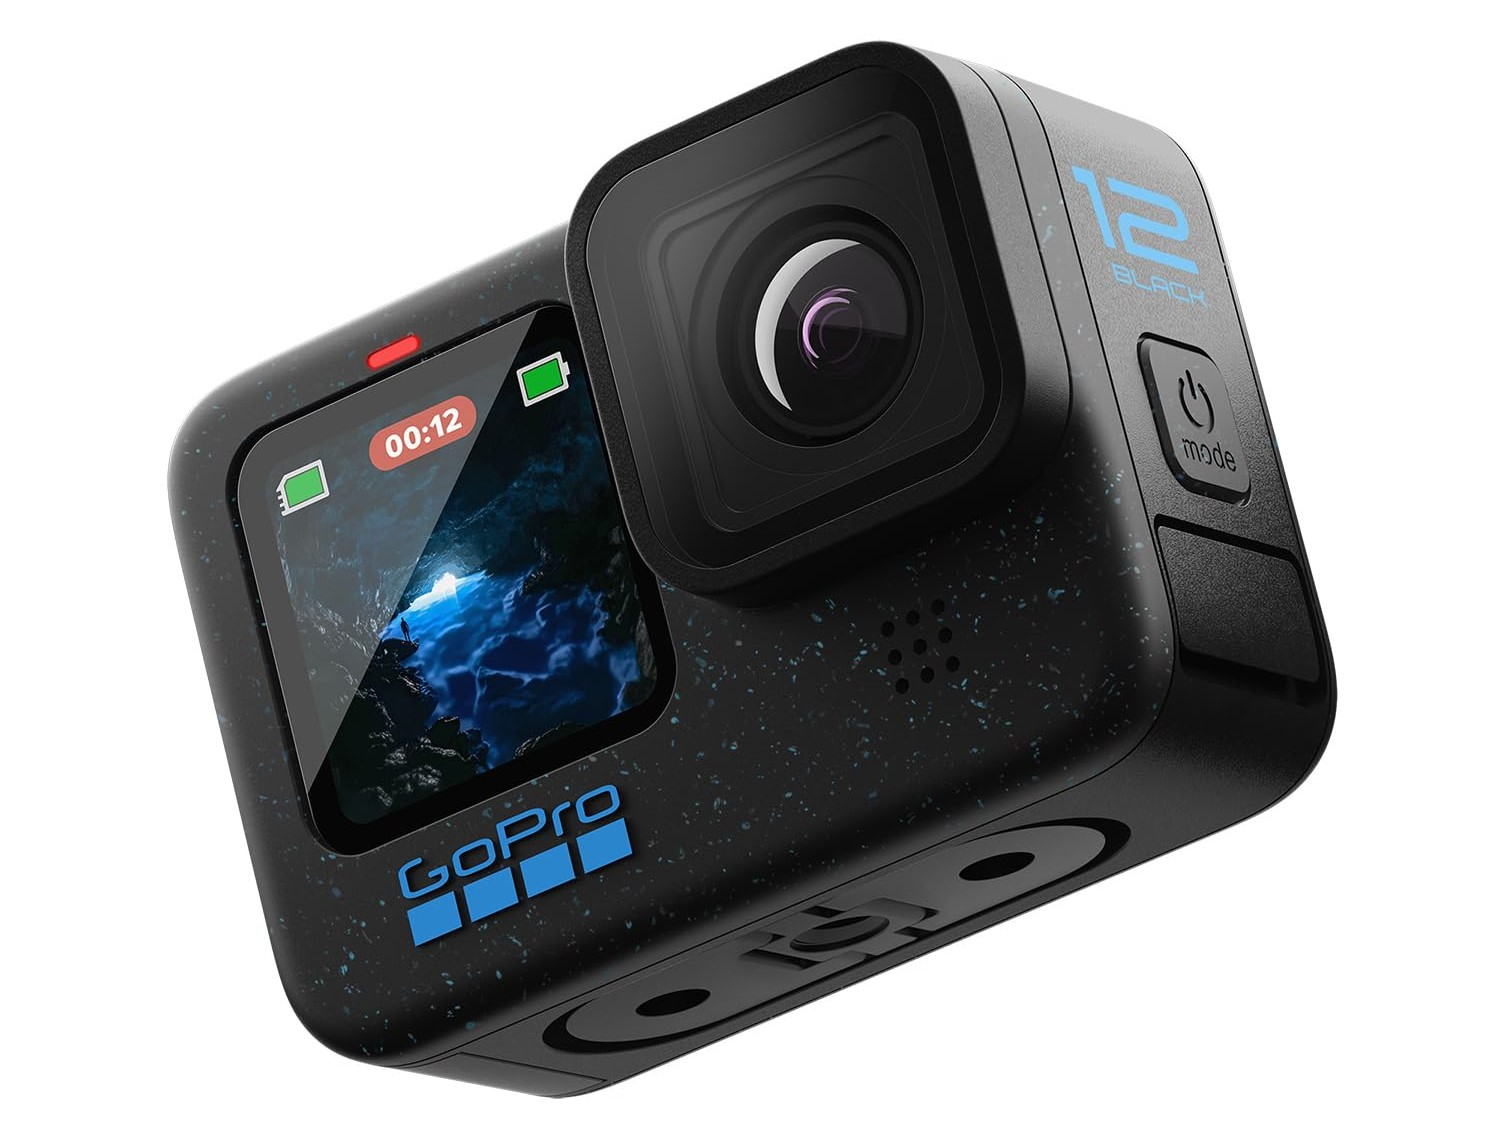
\includegraphics[width=0.65\linewidth]{assets/Capture d'écran process/general/gopro.jpg}
        \caption{Caméra GoPro Héro 12 Black}
        \label{fig:gopro}
    \end{figure}

        Grâce à la plateforme TSS, il a été possible d'accéder au système de référence Vicon/Nexus. C'est un système de motion capture avec marqueurs incluant :
        \begin{itemize}
            \item 18 caméras MXT160
            \item 12 caméras Bonita 3
            \item 7 caméras Vantage 5
            \item baguette de calibration à LED.

        \end{itemize}

        \subsection{Software}
            \subsubsection{Structure de fichiers}
            Pour organiser les données de chaque expérience, une structure de fichiers claire et intuitive a été mise en place :
            \begin{itemize}
                \item \textbf{fichier .pickle:} pour stocker les paramètres de calibration intrinsèques de chaque caméra
                \item \textbf{fichier .hdf5:} pour stocker l'ensemble des paramètres de calibration (intrinsèques et extrinsèques) de chaque caméra après calibration
                \item \textbf{fichier .json:} pour stocker les points 2D détectés par le modèle d'IA pour chaque caméra et les paramètres du projet
                \item \textbf{fichier .csv:} pour stocker les coordonnées 3D triangulées du modèle final
                \item \textbf{fichier .log:} pour stocker les logs générés durant chaque étape du processus MoCapIA
                \item \textbf{fichier .mp4:} pour stocker les vidéos capturées par chaque caméra durant l'expérience
                \item \textbf{fichier .trc:} pour stocker les données 3D - types de fichiers acceptés par OpenSim contrairement aux fichiers CSV
                \item \textbf{fichier .osim:} pour stocker le modèle osseux calculé par le package opensim
                \item \textbf{fichier .mot:} pour stocker les angles articulaires calculés par la \textit{cinématique inverse} d'OpenSim
                \item \textbf{fichier .xml:} pour stocker les paramètres de \textit{scaling} et de \textit{cinématique inverse} d'OpenSim
            \end{itemize}

            \subsubsection{Logiciel}
                \begin{itemize}
                    \item OpenSim 4.5 : pour l'analyse biomécanique du modèle 3D (scaling, cinématique inverse)
                    \item Visual Studio Code : pour le développement en Python et l'écriture du rapport
                    \item Anaconda : pour la gestion des environnements Python et des dépendances
                    \item Git et GitLab UTC : pour le versionnage du code source et la collaboration entre les stagiaires
                    \item GoPro Quik : application Android pour la gestion et la synchronisation des caméras GoPro
                    \item MATLAB : pour la majorité des tests et des analyses d'erreurs
                    \item Notion : pour la prise de notes et le suivi personnel du projet
                \end{itemize}

            \subsubsection{Langage de Programmation}
                \begin{itemize}
                    \item Python 3.8.19 : pour le développement du logiciel MoCapIA (version utilisée par les précédents stagiaires)
                    \item Python 3.10.18 : pour le développement de la partie OpenSim (le changement d'environnement est nécessaire pour la compatibilité avec le package OpenSim mais cela reste automatique)
                    \item Python 3.11.14 : pour le développement de SAM 3D
                    \item Langage MATLAB R2023b
                    \item Langage Latex : pour la rédaction du rapport de stage
                \end{itemize}

        \subsection{FabLab}
        De plus, par la proximité avec le FabLab, il a été possible de créer des pièces sur mesures pour les besoins et les différentes expériences menées durant le projet. Des damiers de calibration de différentes tailles ont été imprimés pour un test sur leur impact sur la qualité de la calibration. Un robot articulé UR3 a été utilisé pour simuler des mouvements précis et répétables lors des tests de calibration.
        \begin{figure}[H]
            \centering
            \begin{subfigure}[b]{0.48\textwidth}
                \centering
                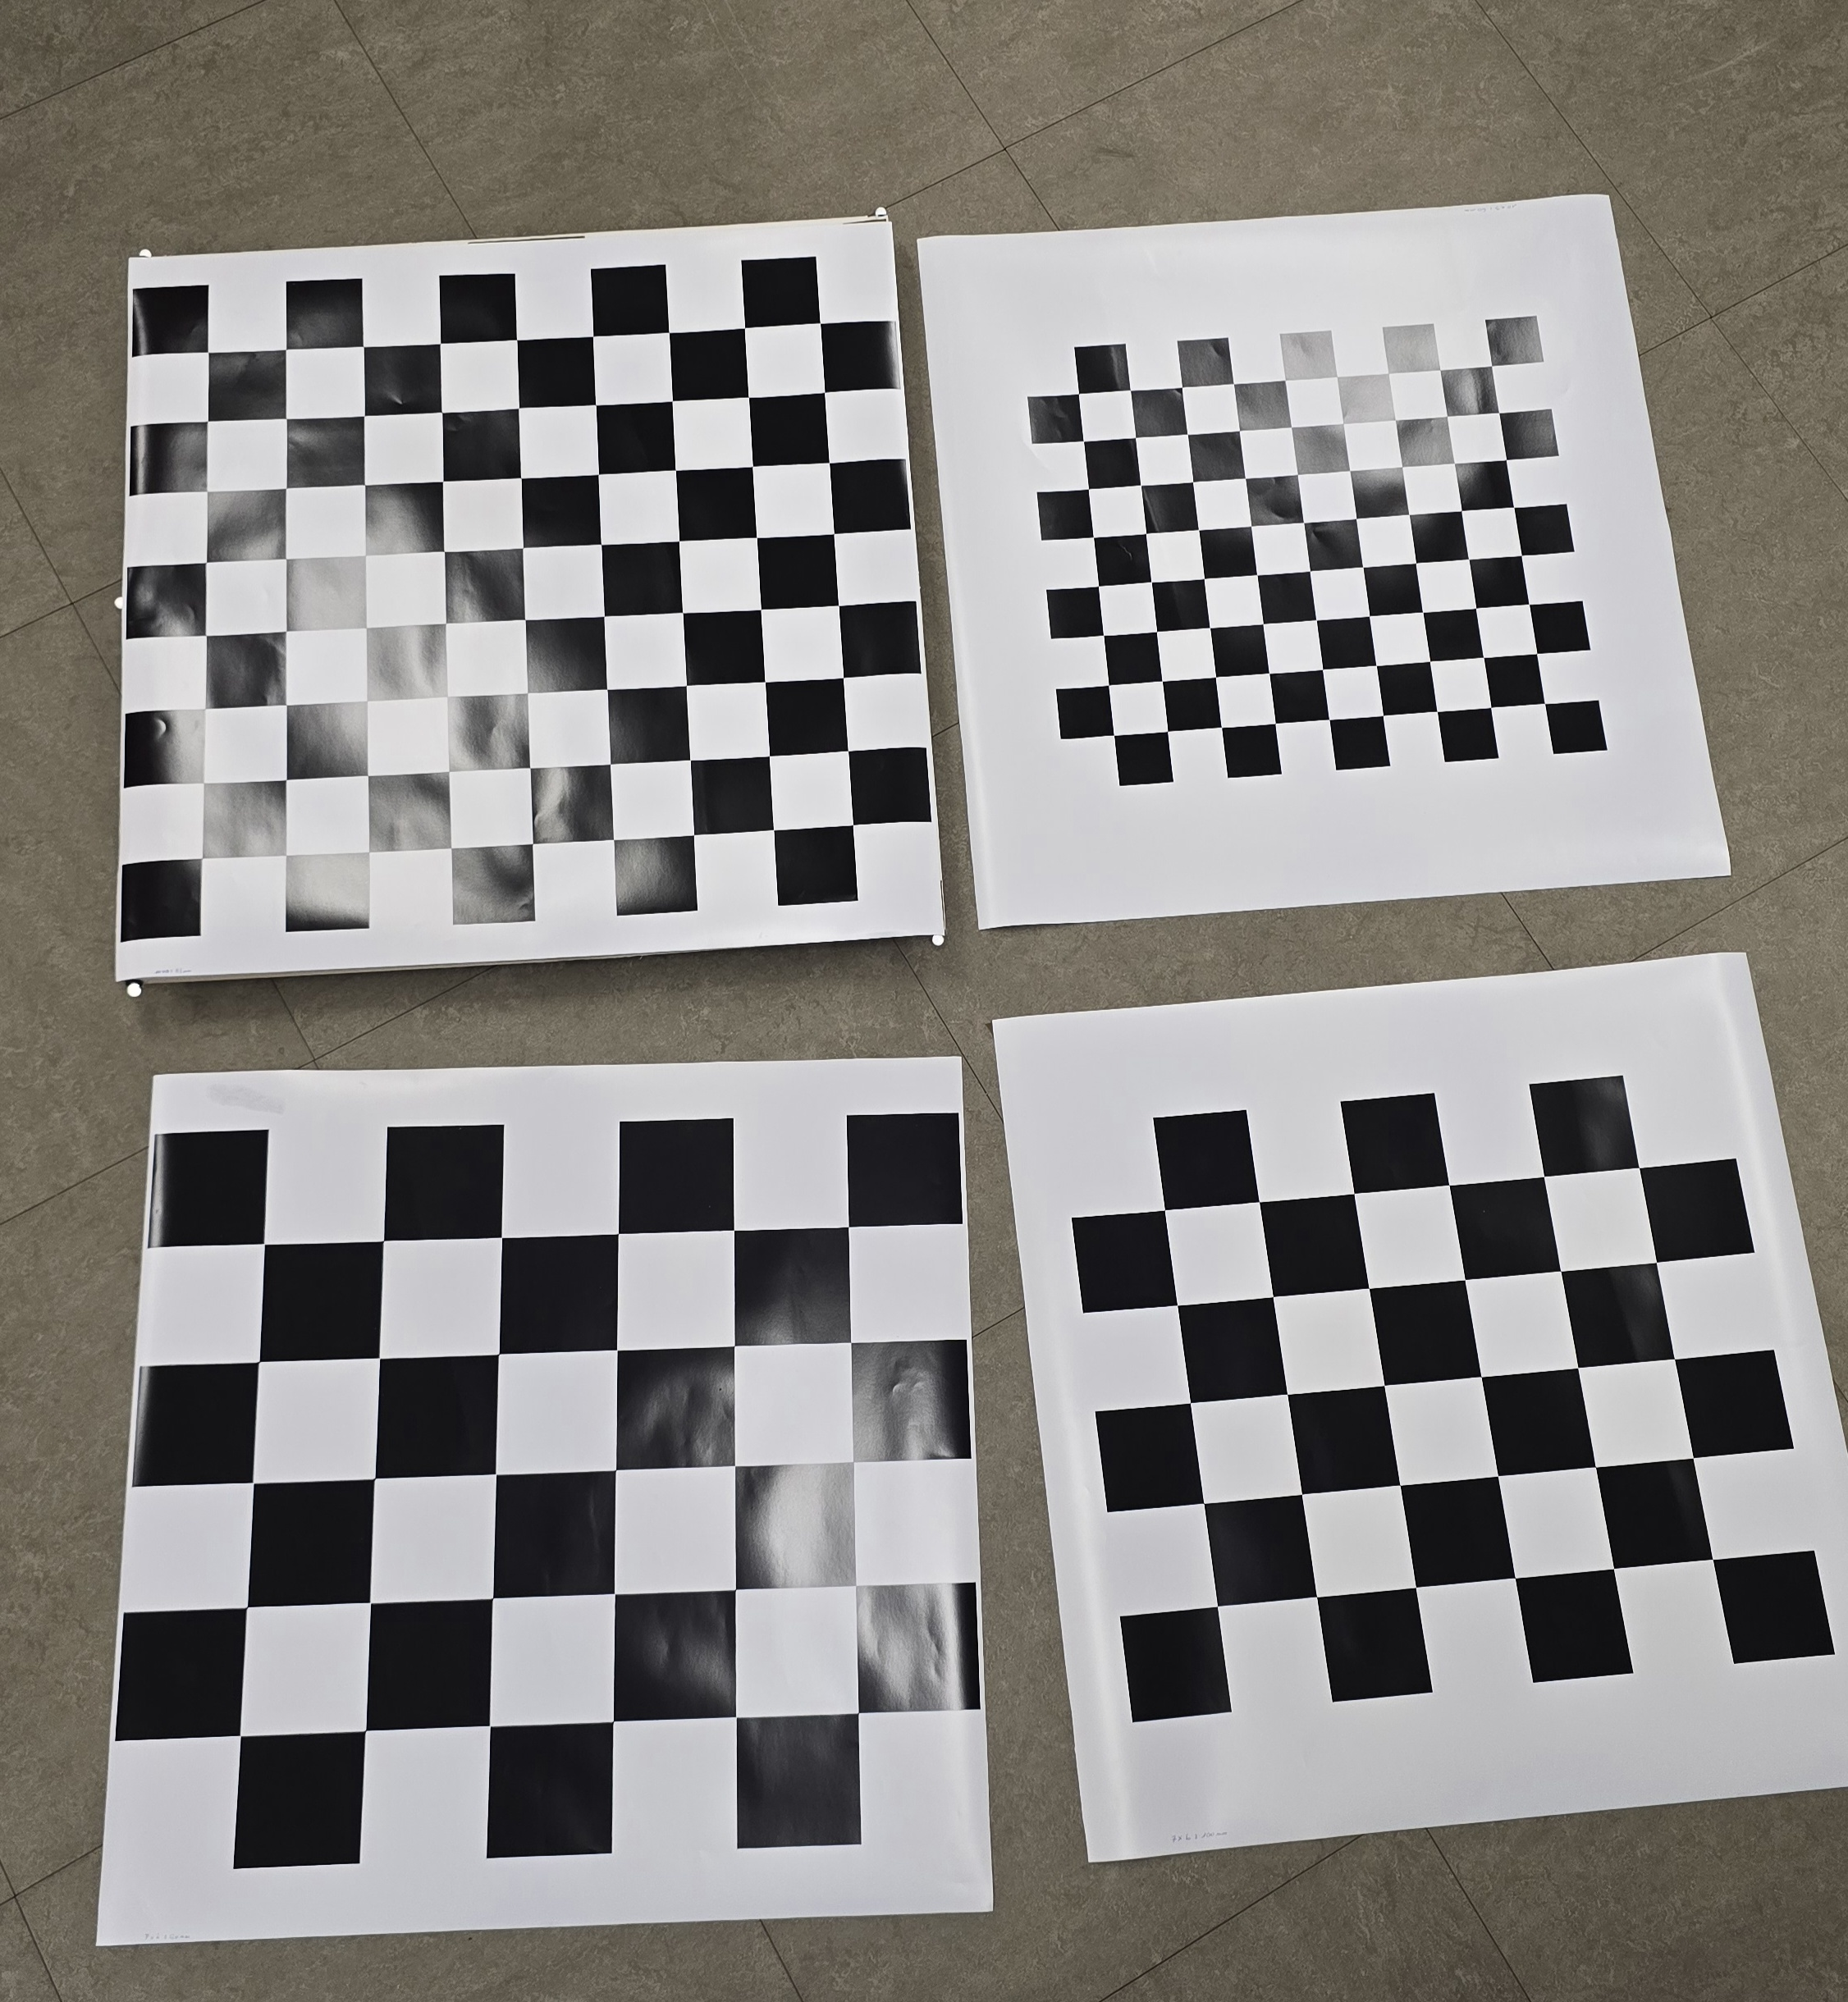
\includegraphics[width=\linewidth]{assets/Capture d'écran process/Test_Damiers/damiers_imprimés.jpg}
                \caption{Damiers de calibration imprimés}
                \label{fig:damiers_fablab}
            \end{subfigure}
            \hfill
            \begin{subfigure}[b]{0.48\textwidth}
                \centering
                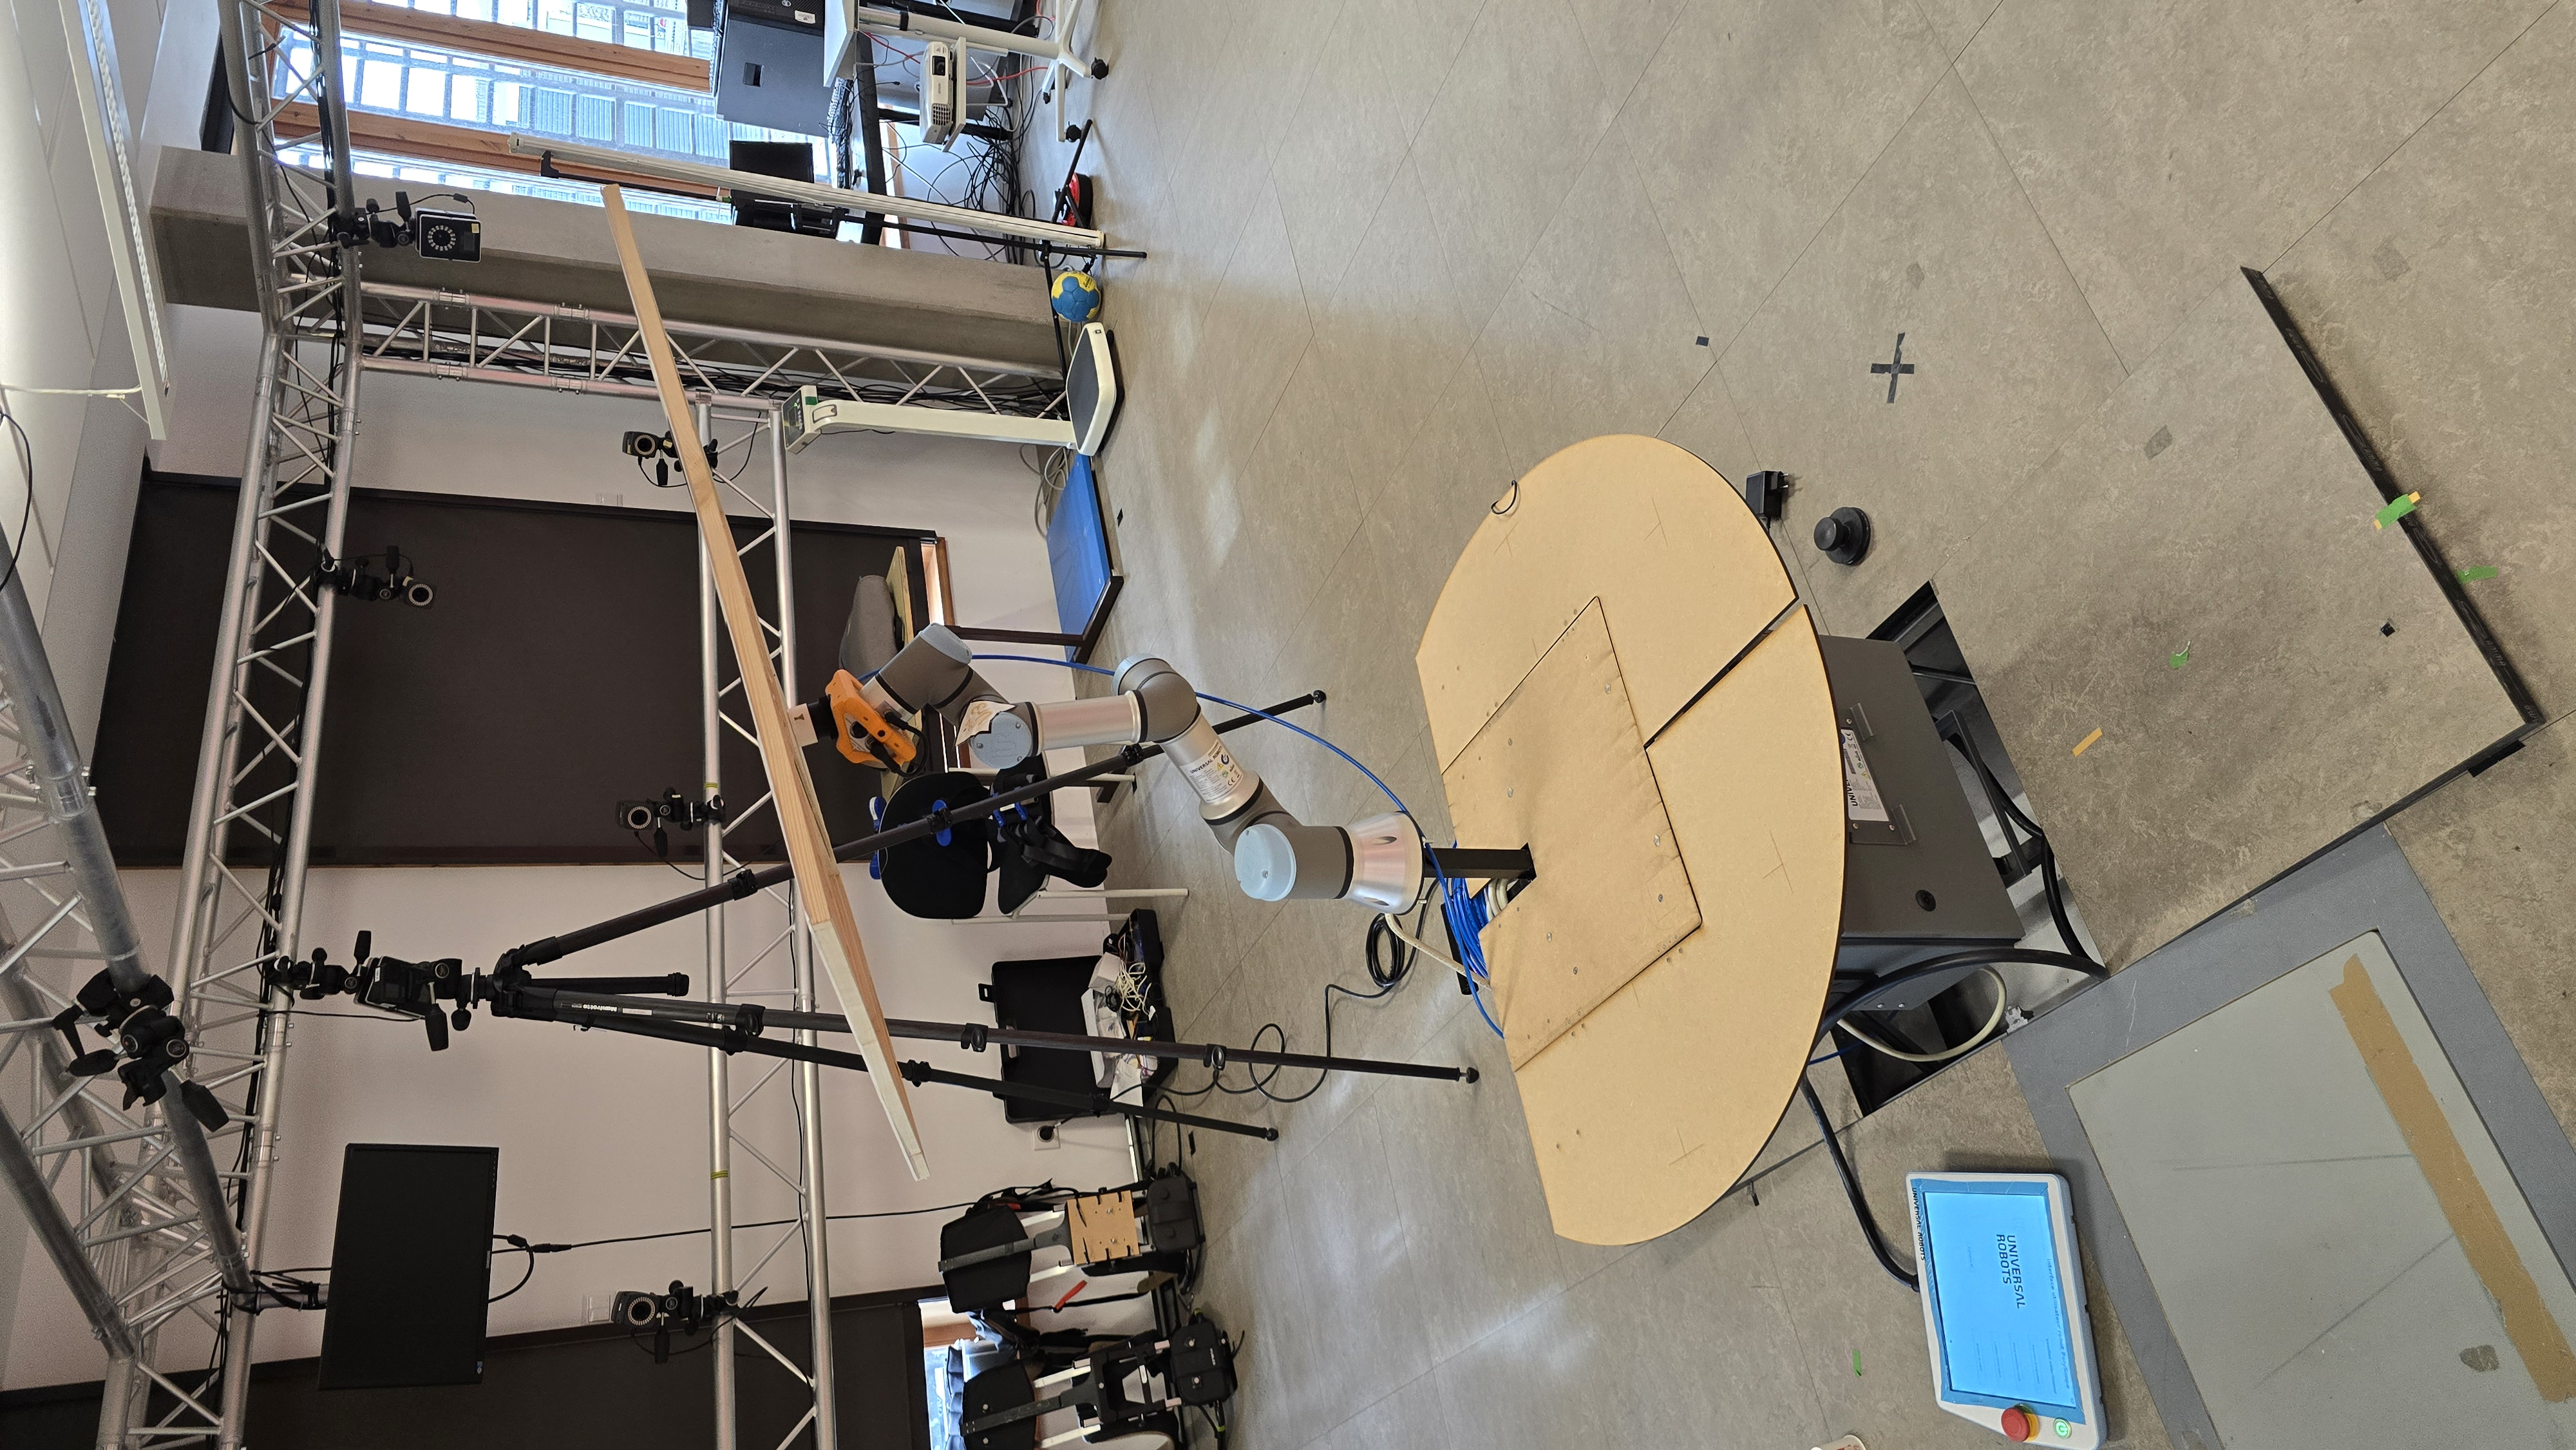
\includegraphics[width=\linewidth, angle=-90]{assets/Capture d'écran process/Test_Damiers/robot.jpg}
                \caption{Robot articulé de test}
                \label{fig:robot_articulé}
            \end{subfigure}
            \caption{Matériel utilisé pour le test sur l'impact des damiers sur la calibration}
            \label{fig:materiel_tests}
        \end{figure}